%%%%%%%%%%%%%%%%%%%%%%%%%%%%%%%%%%%%%%%%%
% APA Assignment Article
% LaTeX Template
% Version 2.0 (February 7, 2023)
%
% This template originates from:
% https://www.LaTeXTemplates.com
%
% Author:
% Vel (vel@latextemplates.com)
%
% License:
% CC BY-NC-SA 4.0 (https://creativecommons.org/licenses/by-nc-sa/4.0/)
%
% NOTE: The bibliography needs to be compiled using the biber engine.
%
%%%%%%%%%%%%%%%%%%%%%%%%%%%%%%%%%%%%%%%%%

%----------------------------------------------------------------------------------------
%	PACKAGES AND OTHER DOCUMENT CONFIGURATIONS
%----------------------------------------------------------------------------------------

\documentclass[
	letterpaper, % Paper size, use either a4paper or letterpaper
	10pt, % Default font size, can also use 11pt or 12pt, although this is not recommended
	unnumberedsections, % Comment to enable section numbering
	twoside, % Two side traditional mode where headers and footers change between odd and even pages, comment this option to make them fixed
]{APAAssignment}

\addbibresource{bibliography.bib} % BibLaTeX bibliography file

\runninghead{MICS CYBER 252, Fall-2024 Hands On Lab 2} % A shortened article title to appear in the running head, leave this command empty for no running head

\footertext{\textit{Hands On Lab 2 (2.5.2)  } (MICS CYBER 252, Fall -2024)} % Text to appear in the footer, leave this command empty for no footer text

\setcounter{page}{1} % The page number of the first page, set this to a higher number if the article is to be part of an issue or larger work

%----------------------------------------------------------------------------------------
%	TITLE SECTION
%----------------------------------------------------------------------------------------

\usepackage[title,toc,titletoc]{appendix}
\usepackage{titlesec}
\usepackage{lscape}
\usepackage{fontawesome}

\title{Hands-On lab 2 \\ MICS-252, Fall 2024} % Article title, use manual lines breaks (\\) to beautify the layout

% Authors are listed in a comma-separated list with superscript numbers indicating affiliations
% \thanks{} is used for any text that should be placed in a footnote on the first page, such as the corresponding author's email, journal acceptance dates, a copyright/license notice, keywords, etc
% Affiliations are output in the \date{} command
\date{UC Berkleley School of Information \\
MICS Course 252 Fall 2024 (Kristy Westphal)
}


\author{
	Prepared by: Karl-Johan Westhoff \\
	email: \href{mailto:kjwesthoff@berkeley.edu}{kjwesthoff@berkeley.edu}
}


% % Full-width abstract
% \renewcommand{\maketitlehookd}{%
% 	\begin{abstract}
% 		\noindent Lorem ipsum dolor sit amet,rta porttitor.
% 	\end{abstract}
% }

%----------------------------------------------------------------------------------------

\setcounter{tocdepth}{5}
\setcounter{secnumdepth}{5}
\usepackage[title]{appendix}

\begin{document}
\onecolumn
\maketitle % Output the title section

%----------------------------------------------------------------------------------------
%	ARTICLE CONTENTS
%----------------------------------------------------------------------------------------

\section{Introduction}
I went through the webGoat exercises and managed to solve most of them, I extensively used the walkthroughs in \cite{CycubicsDocsWebGoat}.
I couldn't get the quiz parts to work and some of the exercised were apparently not working properly for example: 
\begin{itemize}

\item{The last of the JWT exercised reported in Appendix \ref{app:jwtTokens} were in 2 versions (I think), of which I could only solve one, see Appendix \ref{app:JWT1618}}.  
\item{The Pasword reset link exersize Appendix \ref{app:pwReset}, I did get the link redirect to work, but the reset endpoint itself seems to be broken (it also gave me problems using my own credentials)} 
\end{itemize}

\section{Lessons Learned}
Of the exercises I worked with this week, 3 stood out:
\begin{itemize}
	\item{Insecure Login, JWT tokens exercise 16/18, Reported in Appendix \ref{app:JWT1618}, where the header properties of a JWT are defined dynamically, in this case including a SQL injection vulnerability. Lesson learned: More complexity creates more vulnerabilities}
	\item{Insecure Login, password reset, (reported in Appendix \ref{app:pwReset6}) was interesting. Lesson Learned: Do not trust any user inputs (in this case user controlled input was used to generate a link endpoint)}
	\item{Vuln. and Outdated Components, the CVE-2013-7285 (XStream) exercise (reported in Appendix \ref{app:XStrem}). Lesson Learned: Supply chain vulnerabilities, and need for caution when importing and using 3rd party libraries}
\end{itemize}

\section{Topics for Further Exploration}
Topics Here

JWT token exploitation


\subsection{Open source and supply chain vulnerabilities}
Library dependencies and open source
Log4j
tar.xz
openssh

Comment:
Some organizations prefer to have 'someone to blame' and if they paid for proprietary software they feel that they can unload some liability.


\section{Conclusion}
Conclusion Here

%----------------------------------------------------------------------------------------
%	 REFERENCES
%----------------------------------------------------------------------------------------
\clearpage
\printbibliography % Output the bibliography

%----------------------------------------------------------------------------------------



%----------------------------------------------------------------------------------------
%	 Appendices
%----------------------------------------------------------------------------------------

\appendix


\clearpage
\chapter{Appendices}
\begin{appendices}


%\hypertarget{webgoat-setup}{%

\section{Identity and Authentication Failure}}\label{app:AuthAndFailure}
\subsection{Authentication Bypass}
There is  a bug in the password reset system, changing the names in the http POST payload solves the assignment, see Figure \ref{fig:app:AuthBypass}   

\begin{figure}[!ht] % Single column figure
	\centering
	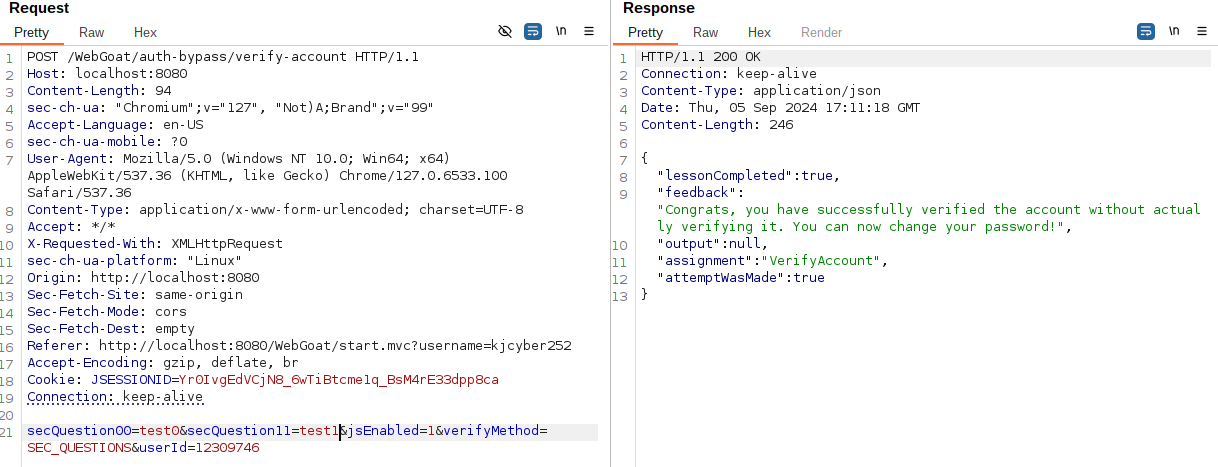
\includegraphics[width=\linewidth]{IdentAndAuthBypass.png}
	\caption{Authentication reset bypassed by changing the secQuestion names the POST request payload}
	\label{fig:app:AuthBypass}
\end{figure}

\subsection{Insecure Login}
For some reason some credentials are hardcoded or left from previous logins when sending the POST request empty, see Figure \ref{fig:app:InsecureLogin}.

\begin{figure}[!ht] % Single column figure
	\centering
	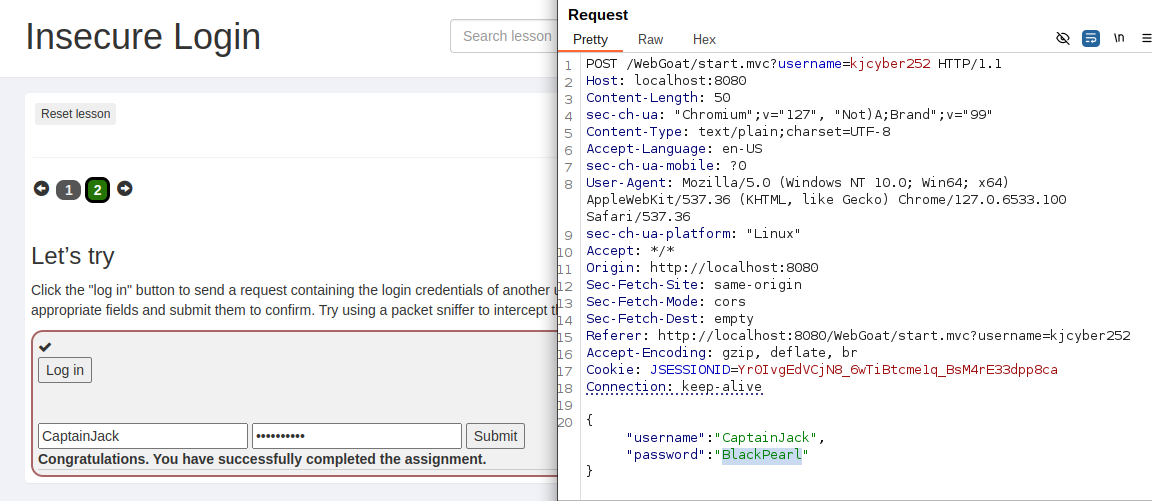
\includegraphics[width=\linewidth]{InsecureLogin.png}
	\caption{Captain Jacks credentials in the POST}
	\label{fig:app:InsecureLogin}
\end{figure}

\subsection{JWT Tokens}\label{app:jwtTokens}
JWT tokens are sometimes used in place of authentication cookies, i.e. without the cross reference protections the browser offers. JWT's are basically ways to send information verified by signatures. In this case the header can be manipulated not to do the verification and blindly trust the token.

\subsubsection{JWT(4)}
Decoded the token on jwt.io and found 'user' as the name

\subsubsection{JWT(6)}
Decoded and manipulated the token using Burps Decoder , setting the signature alg to 'none' and admin to true and got "something" accepted 202, see Figure \ref{fig:app:JWT6} I am not sure this was the intent of the exercise, but it is how far i got.  

\begin{figure}[!ht] % Single column figure
	\centering
	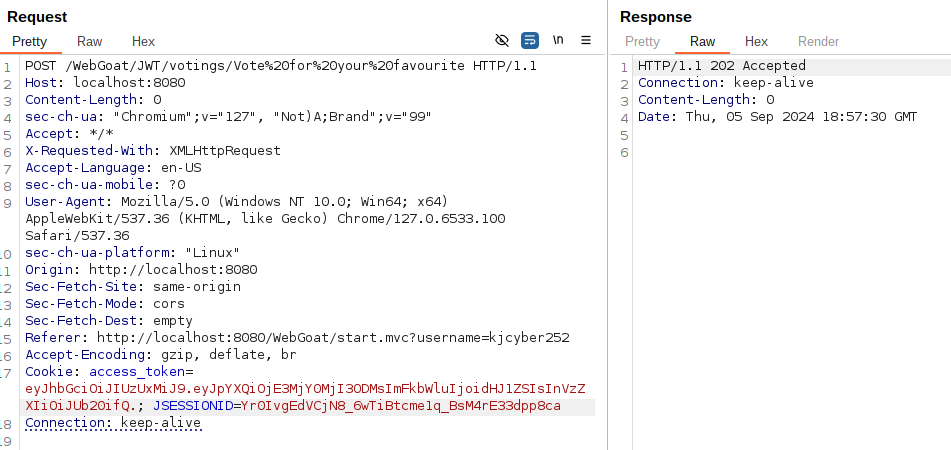
\includegraphics[width=\linewidth]{JWT6.png}
	\caption{JWT token manipulations}
	\label{fig:app:JWT6}
\end{figure}

\subsubsection{JWT(8)}
I was unable to load the Quiz..


\subsubsection{JWT(11)}
JWT Cracking, decided to skip this exercise, intent was to use hashcat and wordlists to break the sha code, but I do not have the tools installed in the machine used for WebGoat.. 


\subsubsection{JWT(13) Refresh Tokens}
Manipulated the token by setting the algorithm to 'none' and manipulating the expiation, see Figure \ref{fig:app:JWT13}

\begin{figure}[!ht] % Single column figure
	\centering
	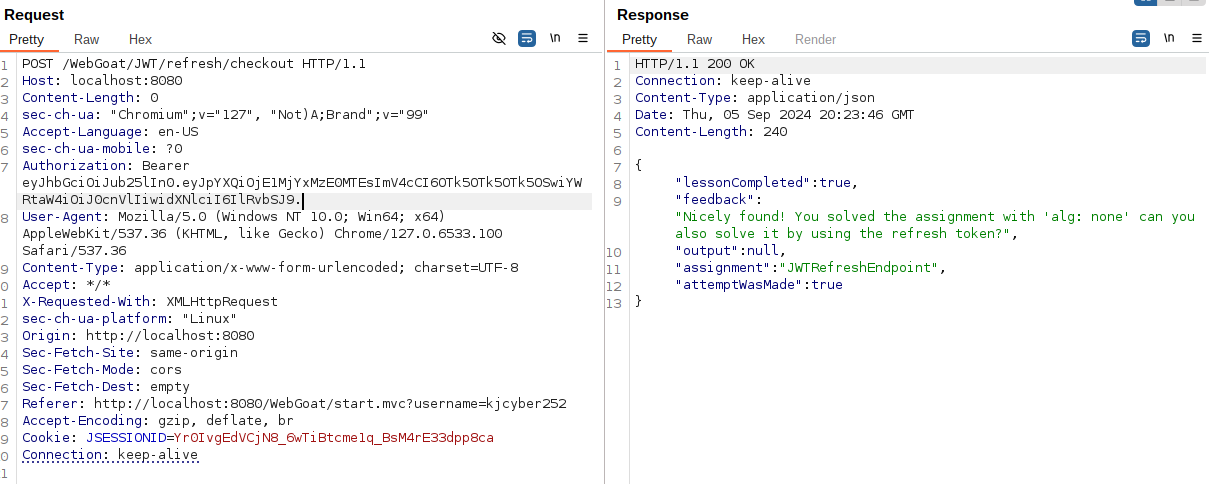
\includegraphics[width=\linewidth]{JWT13_1.png}
	\caption{JWT token manipulations, without refresh.. see next}
	\label{fig:app:JWT13}
\end{figure}


\subsubsection{JWT(16/18) Avanced Token generation..}\label{app:JWT1618}
I found this one difficult and relied on a walkthrough from \cite{MediumJWT8}, where references to the WebGoat source code in GitHub was used to solve the assignment. 

\begin{figure}[!ht] % Single column figure
	\centering
	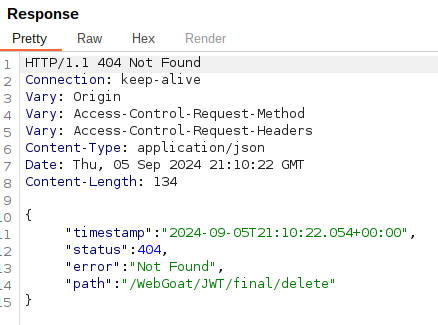
\includegraphics[width=0.5\linewidth]{JWT16_404.png}
	\caption{Could not find the "/WebGoat/JWT/final/delete" endpoint turns out the right page is in 18}
	\label{fig:app:JWT16}
\end{figure}

Manipulated the jwt from the delete POST by changing the names to tom, manipulating expiration and changing the 'kid' to: 
\begin{verbatim}
	"something_else' UNION SELECT 'bmV3X2tleQ==' FROM INFORMATION_SCHEMA.SYSTEM_USERS; --", 
\end{verbatim}

All signed with "new\_key": giving:

\begin{figure}[!ht] % Single column figure
	\centering
	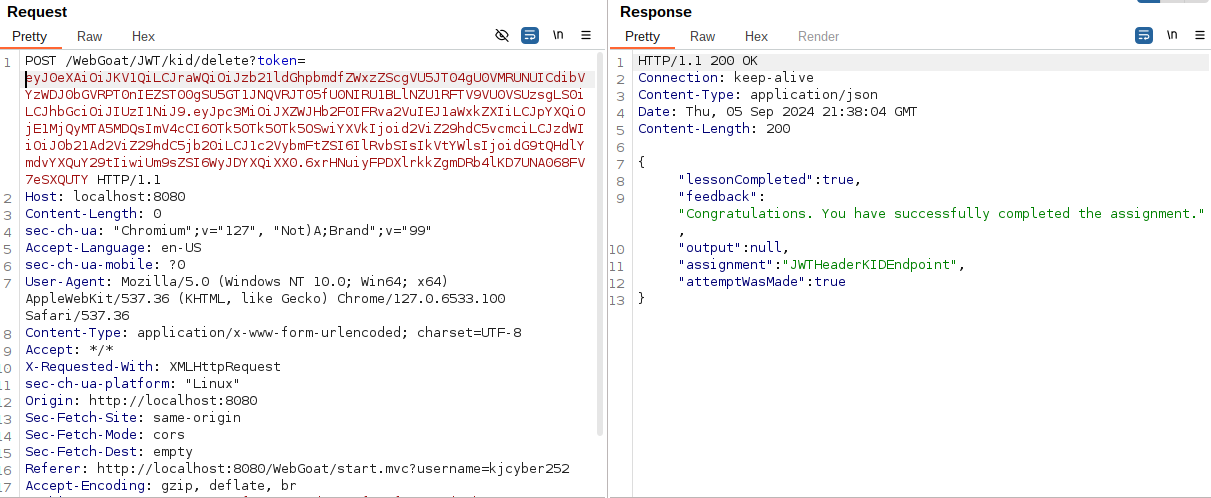
\includegraphics[width=1\linewidth]{JWT_18.png}
	\caption{/WebGoat/JWT/final/delete" Solved!}
	\label{fig:app:JWT18}
\end{figure}

\subsection{Password reset}\label{app:pwReset}

\subsubsection{Password Reset 2: Email functionality with WebWolf}

\begin{figure}[!ht] % Single column figure
	\centering
	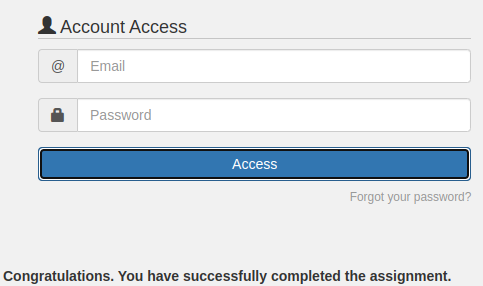
\includegraphics[width=0.5\linewidth]{pw_reset_2.png}
	\caption{Basic password functionality working}
	\label{fig:app:pw_reset_2}
\end{figure}

\subsubsection{Password Reset 4: Security questions}

\begin{figure}[!ht] % Single column figure
	\centering
	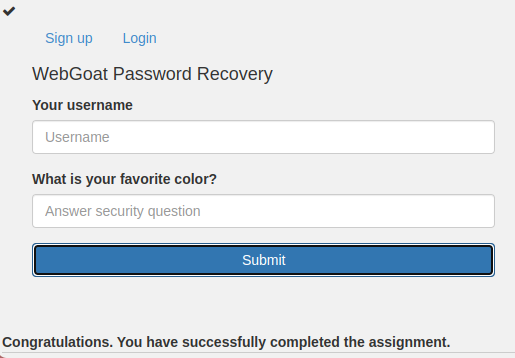
\includegraphics[width=0.5\linewidth]{pw_reset_4.png}
	\caption{Reset challenge questions brute force-able, un:Top, pw:purple (from \cite{CycubicsDocsWebGoat}}
	\label{fig:app:pw_reset_4}
\end{figure}

\subsubsection{Password Reset 5: The Problem with Security Questions}
Will be sure not to implement.


\subsubsection{Password Reset 6: Creating the password reset link}\label{app:pwReset6}

Redirecting the reset password link, the link is generated by a the Host in the POST header (which can be manipulated) and a  random number. The link is sent to whatever email is in the payload see figure \ref{fig:app:pwreset-redirect}. The link is then redirected to WebWolf which we control \ref{fig:app:pwreset-intercept}. Unfortunately i think the reset mechanism is broken, after supplying the reset password, I am directed to an error page. 

\begin{figure}[!htp] % Single column figure
	\centering
	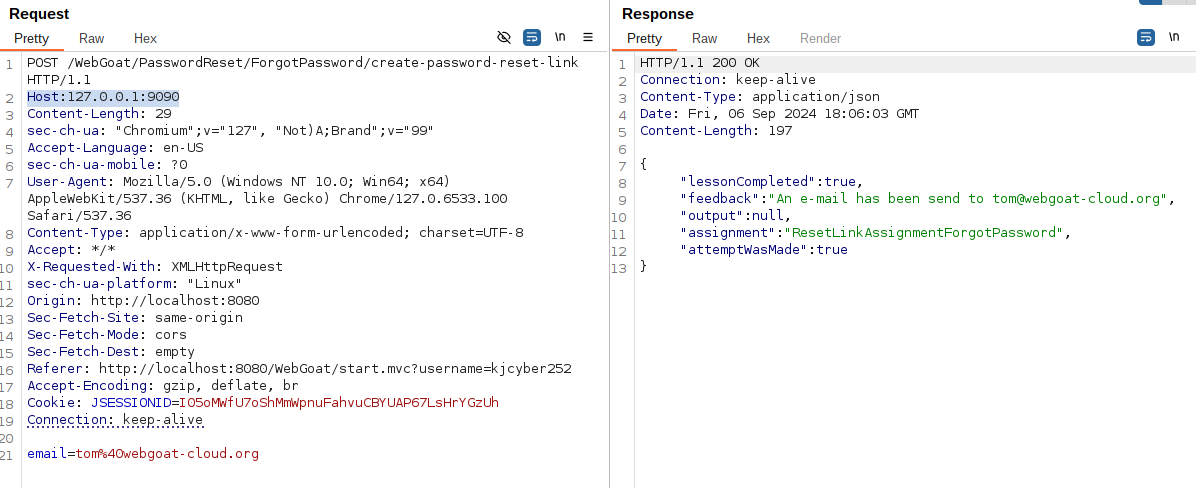
\includegraphics[width=\linewidth]{pw_reset6-redirect.png}
	\caption{Manipulating where the password reset link is sent}
	\label{fig:app:pwreset-redirect}
\end{figure}

\begin{figure}[!htp] % Single column figure
	\centering
	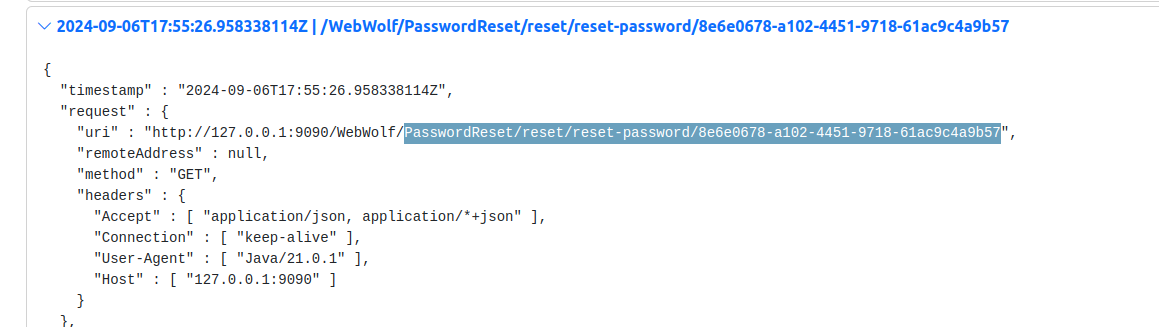
\includegraphics[width=\linewidth]{pw_reset6-intercept.png}
	\caption{Link intercepted in webwolf}
	\label{fig:app:pwreset-intercept}
\end{figure}


\subsection{Secure Passwords}
See Figure \ref{fig:app:SecurePW}

\begin{figure}[!htp] % Single column figure
	\centering
	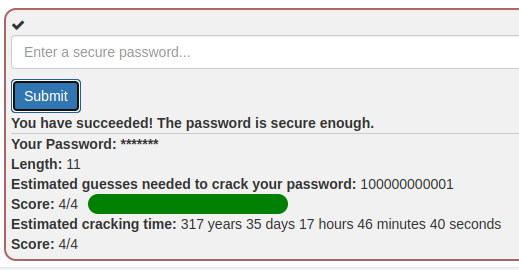
\includegraphics[width=0.5\linewidth]{PasswordStrength.png}
	\caption{Secure Passwords: Following the NIST recommendations}
	\label{fig:app:SecurePW}
\end{figure}


\section{Vuln. and Outdated Components}\label{app:VulnAndOutdatedComponents}
\subsection{(5)The exploit is not always in "your" code}\label{app:VulnAndOutdatedComponents5}

\begin{figure}[!ht] % Single column figure
	\centering
	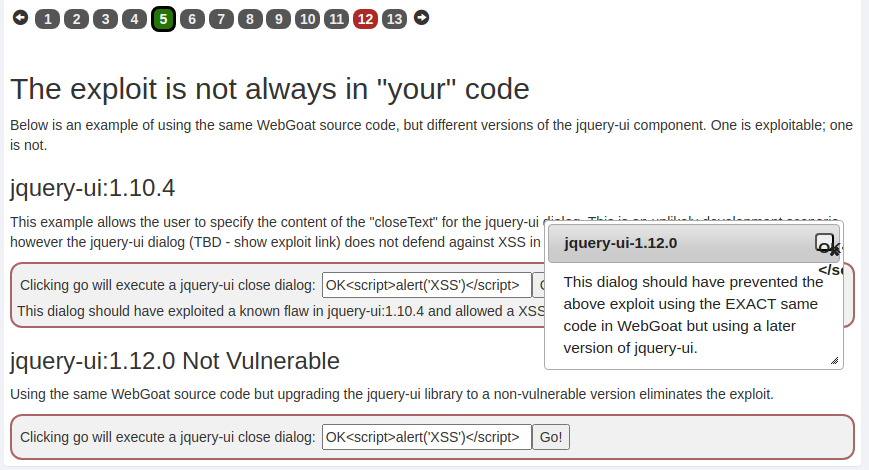
\includegraphics[width=\linewidth]{VulnComponents5.png}
	\caption{Differences in JQuery versions, one of which is vulnerable to reflected XSS }
	\label{fig:app:vuln5}
\end{figure}

\subsection{(12)Exploiting CVE-2013-7285 (XStream)}\label{app:VulnAndOutdatedComponents12}\label{app:XStrem}
This one is scary. XStream is a serial/de-serializer for XML, JSON etc. when used as a deserializer, it opens up possibility of an OS command injection resulting in remote code execution. XStream.fromXML deserializes into an Java Object, vulnerable to OS injection as <interface>org.owasp.webgoat.lessons.vulnerable components.Contact</interface> the Contact function will be executed   

\begin{figure}[!ht] % Single column figure
	\centering
	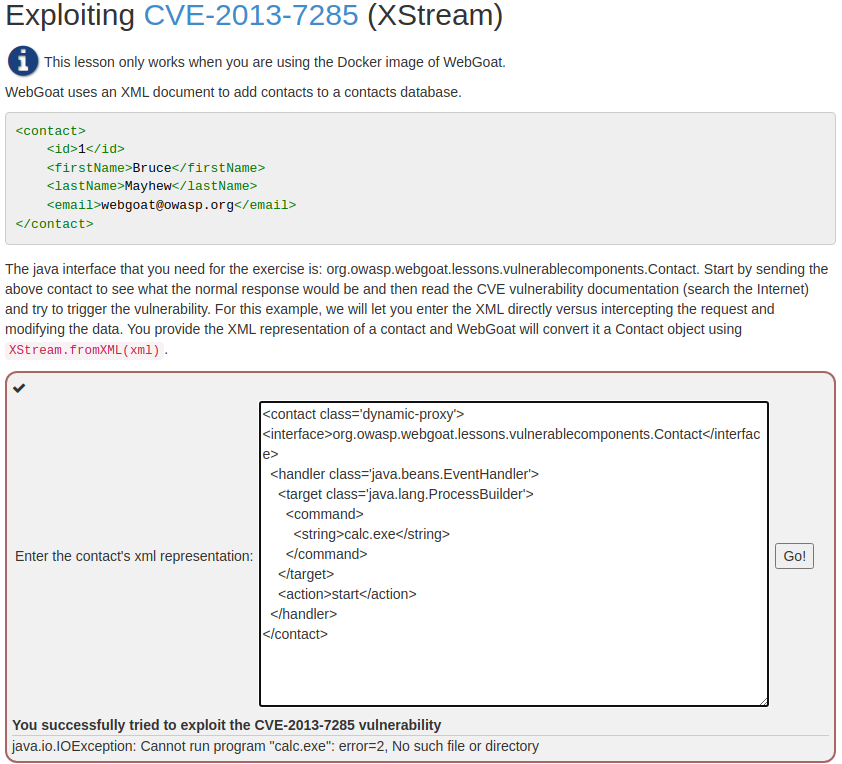
\includegraphics[width=\linewidth]{VulnComponents12.png}
	\caption{XStream deserializes and executes Contact function resulting in remote code execution}
	\label{fig:app:vuln12}
\end{figure}


\begin{figure}[!ht] % Single column figure
	\centering
	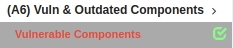
\includegraphics[width=0.3\linewidth]{VulnOutdatedSolved.png}
	\caption{Section A6 Solved}
	\label{fig:app:vulnSolved}
\end{figure}

\section{Security Logging Failures}\label{app:SecurityLogging}
\subsection{Lets Try (2)}
See solved Figure \ref{fig:app:LetsTry}

\begin{figure}[!htp] % Single column figure
	\centering
	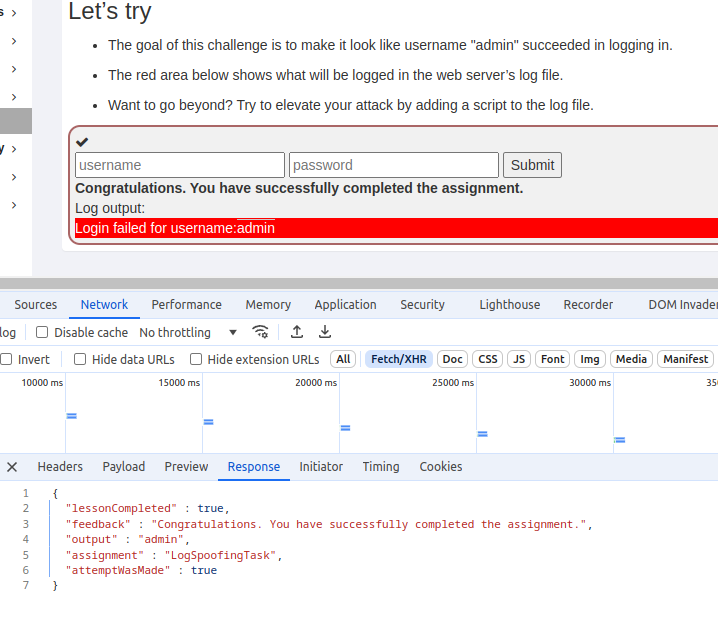
\includegraphics[width=0.3\linewidth]{LetsTry.png}
	\caption{Lets Try solved using inspiration from \cite{CycubicsDocsWebGoat}, username: admin, pw: url encoded Za\%0d\%a}
	\label{fig:app:LetsTry}
\end{figure}

\subsection{Lets Try (4)}
See Figure \ref{fig:app:LogBleeding}

\begin{figure}[!htp] % Single column figure
	\centering
	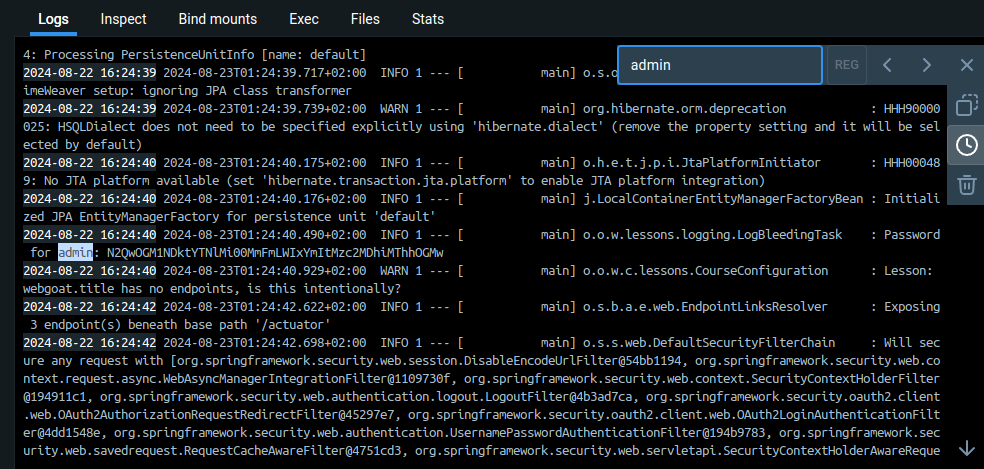
\includegraphics[width=\linewidth]{LogBleeding.png}
	\caption{The Password is leaked, internally on the server (exploitation requires access to the server)}
	\label{fig:app:LogBleeding}
\end{figure}

\section{Client Side}\label{app:ClientSide}

\subsection{Bypass front-end restrictions}
Client Side DOM and JS manipulation

\subsubsection{Field Restrictions}
Bypassed the input fields by manipulating the POST request with impossible options see Figure \ref{fig:app:ClientBypass} 

\begin{figure}[!htp] % Single column figure
	\centering
	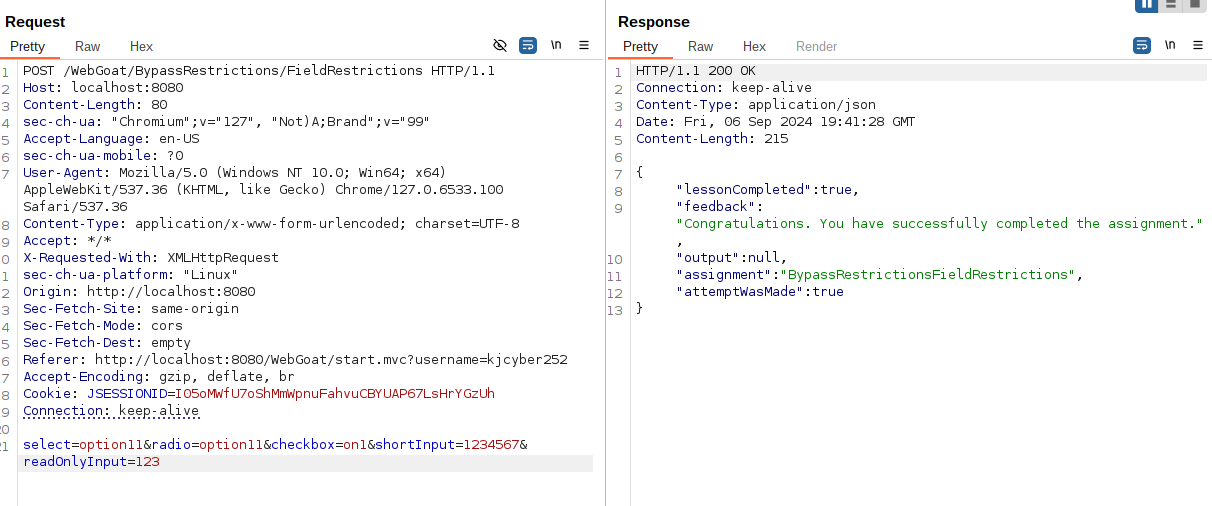
\includegraphics[width=\linewidth]{ClientBypass.png}
	\caption{Bypassed the input fields by manipulating the POST request with impossible options}
	\label{fig:app:ClientBypass}
\end{figure}

\subsubsection{Validation}
See Figure \ref{fig:app:ClientBypas2}

\begin{figure}[!htp] % Single column figure
	\centering
	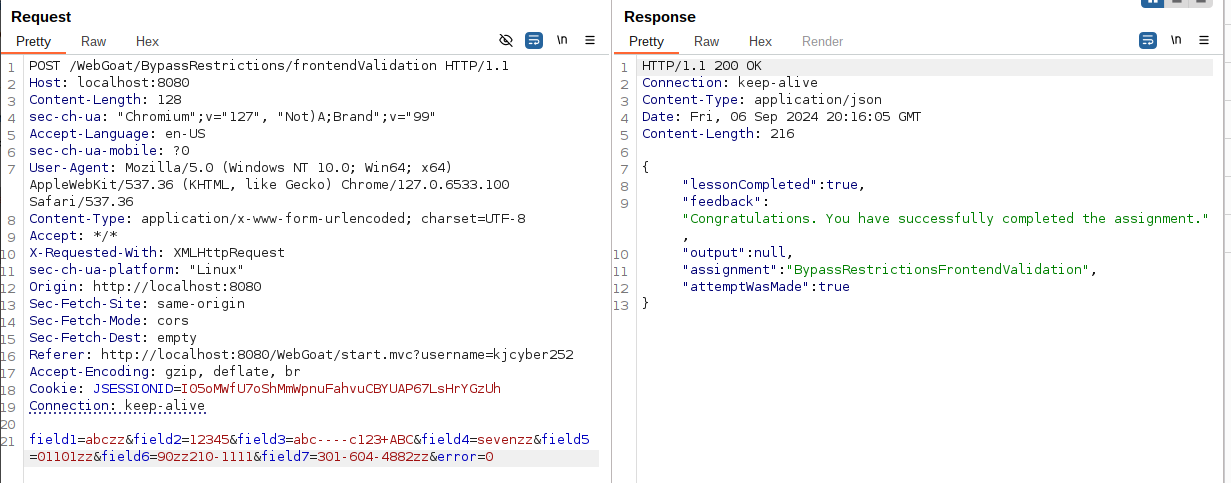
\includegraphics[width=\linewidth]{ClientBypass2.png}
	\caption{Bypassed the input fields by manipulating the POST request with impossible options still works with validation}
	\label{fig:app:ClientBypass2}
\end{figure}

\subsection{Client side filtering}
\subsubsection{Salary manager (2)}
Found Bartholomew's salary in a hidden table in the DOM, see Figure \ref{fig:app:SalaryManager}

\begin{figure}[!htp] % Single column figure
	\centering
	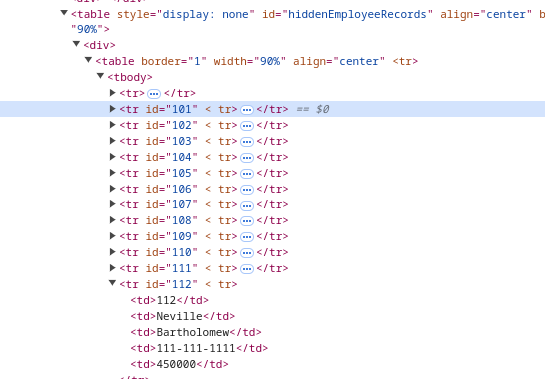
\includegraphics[width=0.5\linewidth]{SalaryManager.png}
	\caption{Found Bartholomew's 450000 salary in a hidden table in the DOM}
	\label{fig:app:SalaryManager}
\end{figure}

\subsubsection{Samsung Galaxy S8}
Filling out the form an looking at Network traffic in the chrome tools, there is an endpoint for the coupons. If a invalid coupon is entered, the server returns a massage, if the field is left empty there is no traffic. If hitting the endpoint anyway, the code is included in the server response,
see Figure \ref{fig:app:samsungResponse}


\begin{figure}[!htp] % Single column figure
	\centering
	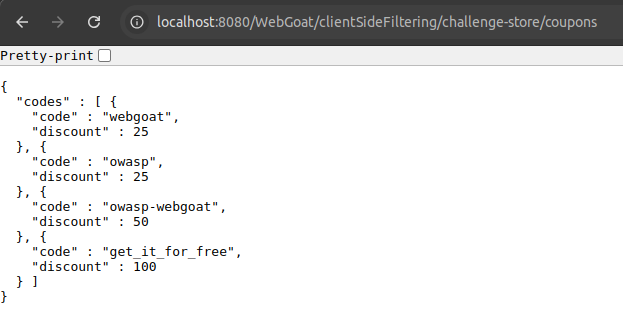
\includegraphics[width=0.5\linewidth]{samsungResponse.png}
	\caption{Found the code in an empty coupon API call}
	\label{fig:app:samsungResponse}
\end{figure}


\subsection{HTML tampering}
See Figure \ref{fig:app:Tampering}
\begin{figure}[!htp] % Single column figure
	\centering
	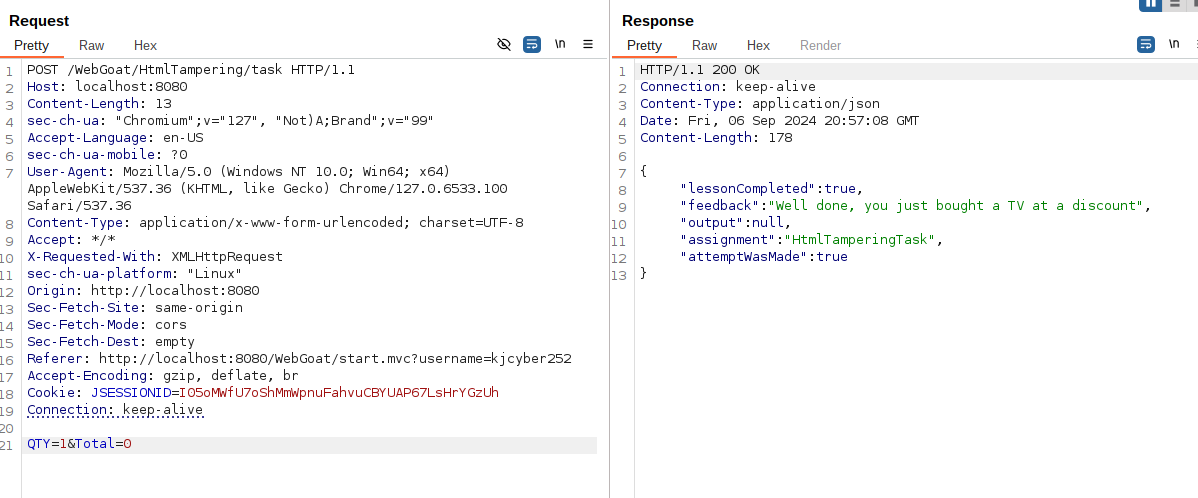
\includegraphics[width=\linewidth]{Tampering.png}
	\caption{Quantity and Amount can be manipulated in the POST Request}
	\label{fig:app:Tampering}
\end{figure}




\end{appendices}
\end{document}
